\documentclass[11pt]{article}
\usepackage[textwidth=18.0cm, textheight=23.0cm, top=2.0cm]{geometry}
\usepackage{pst-all}
\usepackage{amssymb}
\usepackage{tikz}
\usepackage{underscore}\begin{document}
\pagestyle{empty}


ClassName: \underline{\textbf{Class_10.2bp-7}}
\par
BinSize: \underline{\textbf{100 × 100}}
\par
ReduceSize: \underline{\textbf{100 × 100}}
\par
TypeNum: \underline{\textbf{20}}
\par
Num: \underline{\textbf{20}}
\par
OutS: \underline{\textbf{30000}}
\par
InS: \underline{\textbf{19414}}
\par
Rate: \underline{\textbf{0.647}}
\par
UB: \underline{\textbf{3}}
\par
LB0: \underline{\textbf{3}}
\par
LB: \underline{\textbf{3}}
\par
LBWithCut: \underline{\textbf{3}}
\par
NodeCut: \underline{\textbf{0}}
\par
ExtendedNodeCnt: \underline{\textbf{1}}
\par
GenNodeCnt: \underline{\textbf{1}}
\par
PrimalNode: \underline{\textbf{0}}
\par
ColumnCount: \underline{\textbf{3}}
\par
TotalCutCount: \underline{\textbf{0}}
\par
RootCutCount: \underline{\textbf{0}}
\par
LPSolverCnt: \underline{\textbf{1}}
\par
PricingSolverCnt: \underline{\textbf{0}}
\par
BranchAndBoundNum: \underline{\textbf{1}}
\par
isOpt: \underline{\textbf{true}}
\par
TimeOnInitSolution: \underline{\textbf{600.000 s}}
\par
TimeOnPrimal: \underline{\textbf{0.000 s}}
\par
TimeOnPricing: \underline{\textbf{0.000 s}}
\par
TimeOnRmp: \underline{\textbf{0.062 s}}
\par
TotalTime: \underline{\textbf{600.311 s}}
\par
\newpage


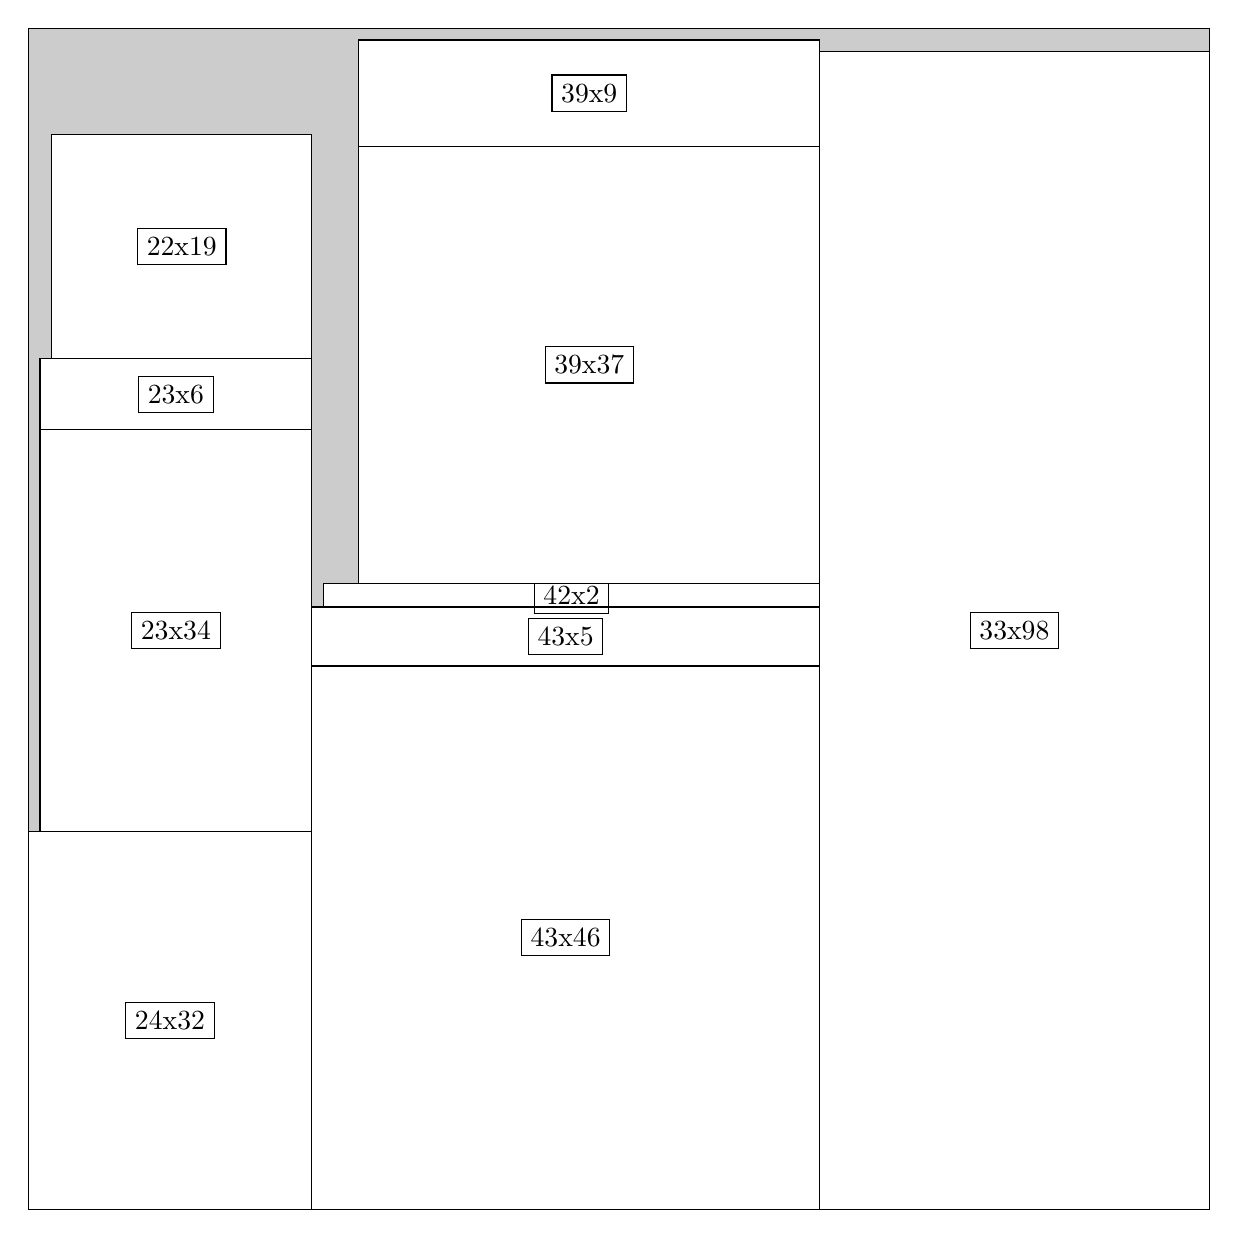
\begin{tikzpicture}[shorten >=1pt,scale=1.0,every node/.style={scale=1.0},->]
\tikzstyle{vertex}=[circle,fill=black!25,minimum size=14pt,inner sep=0pt]
\filldraw[fill=gray!40!white, draw=black] (0,0) rectangle (15.0,15.0);
\foreach \name/\x/\y/\w/\h in {33x98/10.049999999999999/0.0/4.95/14.7,43x46/3.5999999999999996/0.0/6.45/6.8999999999999995,43x5/3.5999999999999996/6.8999999999999995/6.45/0.75,42x2/3.75/7.6499999999999995/6.3/0.3,39x37/4.2/7.949999999999999/5.85/5.55,39x9/4.2/13.5/5.85/1.3499999999999999,24x32/0.0/0.0/3.5999999999999996/4.8,23x34/0.15/4.8/3.4499999999999997/5.1,23x6/0.15/9.9/3.4499999999999997/0.8999999999999999,22x19/0.3/10.799999999999999/3.3/2.85}
\filldraw[fill=white!40!white, draw=black] (\x,\y) rectangle node[draw] (\name) {\name} ++(\w,\h);
\end{tikzpicture}


w =33 , h =98 , x =67 , y =0 , v =3234
\par
w =43 , h =46 , x =24 , y =0 , v =1978
\par
w =43 , h =5 , x =24 , y =46 , v =215
\par
w =42 , h =2 , x =25 , y =51 , v =84
\par
w =39 , h =37 , x =28 , y =53 , v =1443
\par
w =39 , h =9 , x =28 , y =90 , v =351
\par
w =24 , h =32 , x =0 , y =0 , v =768
\par
w =23 , h =34 , x =1 , y =32 , v =782
\par
w =23 , h =6 , x =1 , y =66 , v =138
\par
w =22 , h =19 , x =2 , y =72 , v =418
\par
\newpage


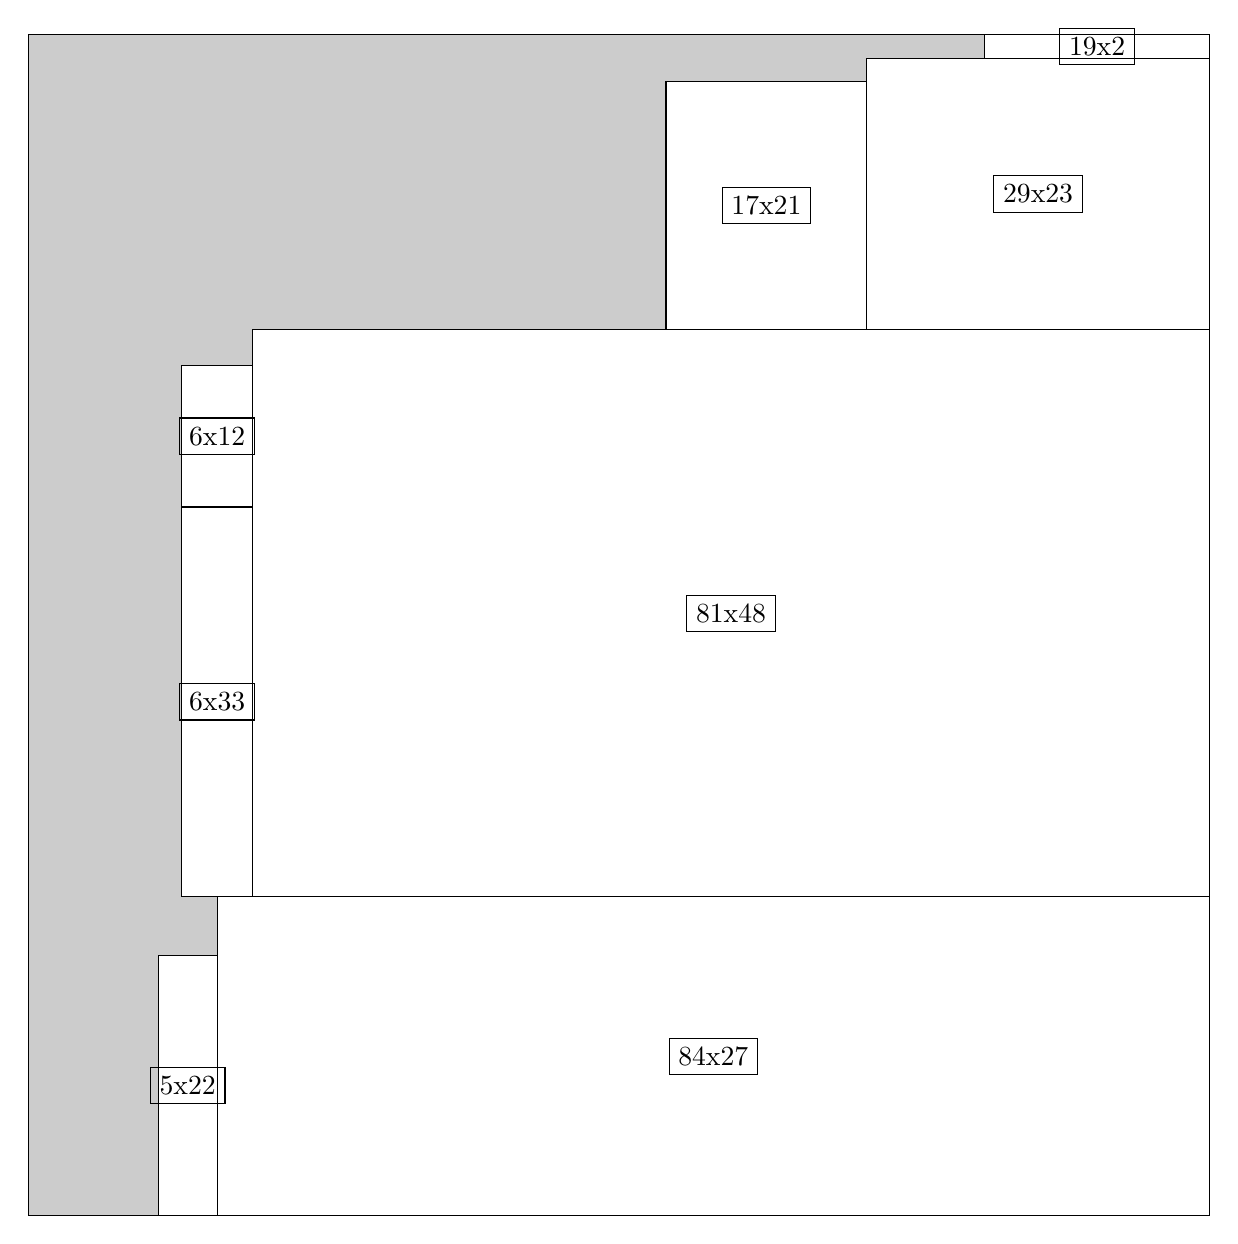
\begin{tikzpicture}[shorten >=1pt,scale=1.0,every node/.style={scale=1.0},->]
\tikzstyle{vertex}=[circle,fill=black!25,minimum size=14pt,inner sep=0pt]
\filldraw[fill=gray!40!white, draw=black] (0,0) rectangle (15.0,15.0);
\foreach \name/\x/\y/\w/\h in {84x27/2.4/0.0/12.6/4.05,5x22/1.65/0.0/0.75/3.3,81x48/2.85/4.05/12.15/7.199999999999999,6x33/1.95/4.05/0.8999999999999999/4.95,6x12/1.95/9.0/0.8999999999999999/1.7999999999999998,29x23/10.65/11.25/4.35/3.4499999999999997,19x2/12.15/14.7/2.85/0.3,17x21/8.1/11.25/2.55/3.15}
\filldraw[fill=white!40!white, draw=black] (\x,\y) rectangle node[draw] (\name) {\name} ++(\w,\h);
\end{tikzpicture}


w =84 , h =27 , x =16 , y =0 , v =2268
\par
w =5 , h =22 , x =11 , y =0 , v =110
\par
w =81 , h =48 , x =19 , y =27 , v =3888
\par
w =6 , h =33 , x =13 , y =27 , v =198
\par
w =6 , h =12 , x =13 , y =60 , v =72
\par
w =29 , h =23 , x =71 , y =75 , v =667
\par
w =19 , h =2 , x =81 , y =98 , v =38
\par
w =17 , h =21 , x =54 , y =75 , v =357
\par
\newpage


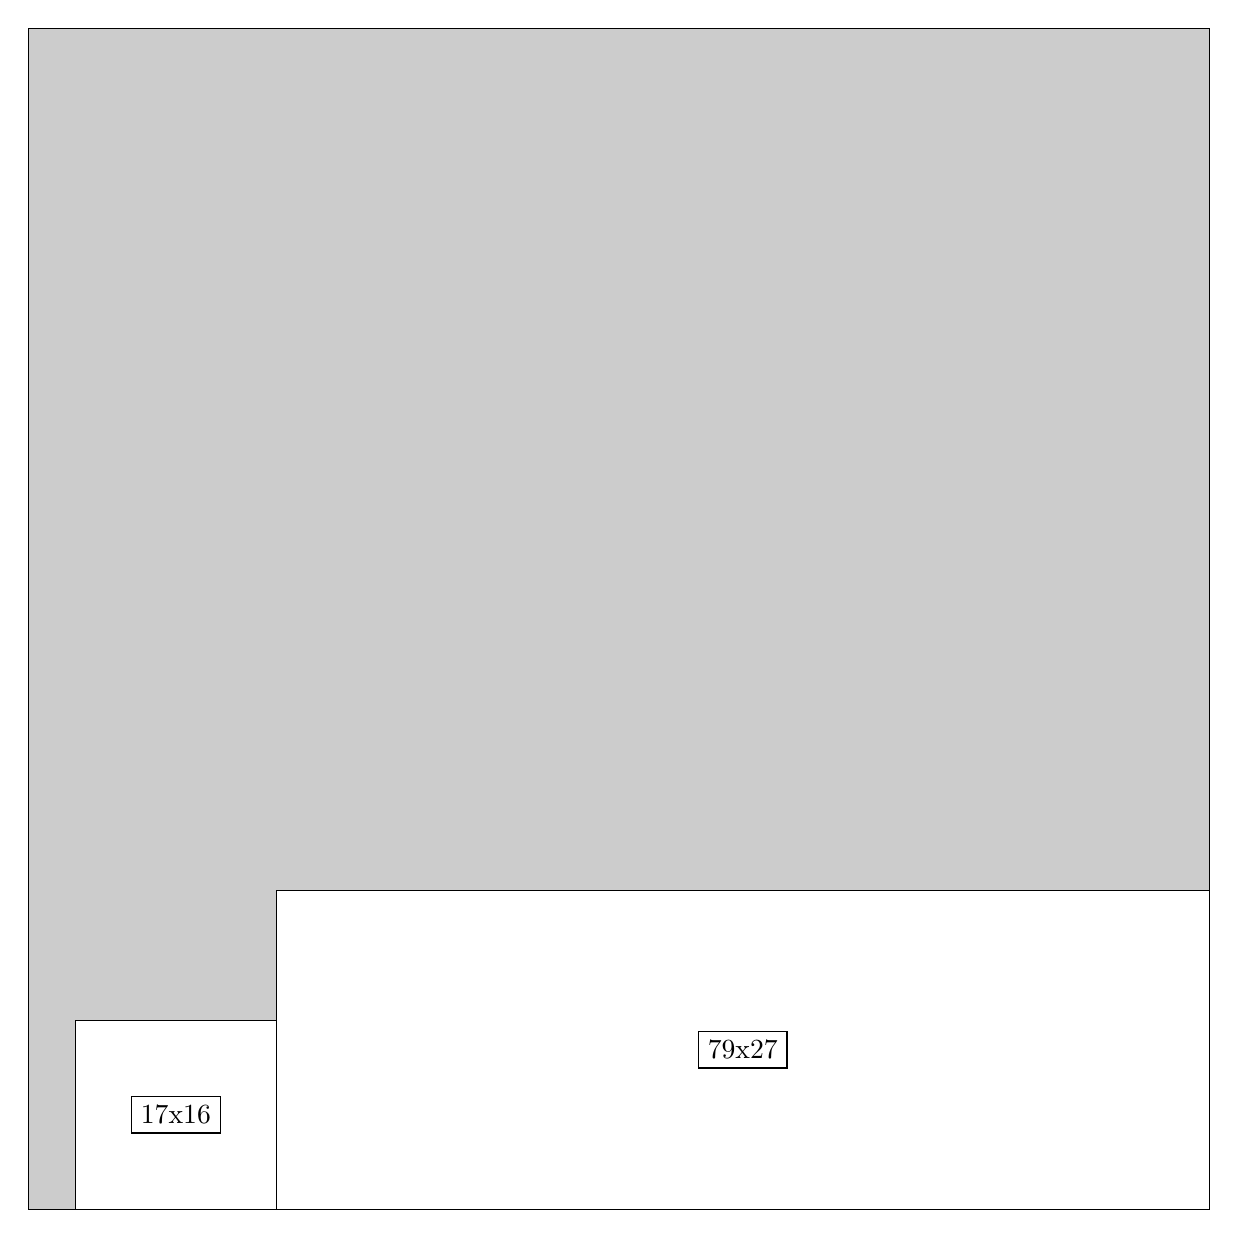
\begin{tikzpicture}[shorten >=1pt,scale=1.0,every node/.style={scale=1.0},->]
\tikzstyle{vertex}=[circle,fill=black!25,minimum size=14pt,inner sep=0pt]
\filldraw[fill=gray!40!white, draw=black] (0,0) rectangle (15.0,15.0);
\foreach \name/\x/\y/\w/\h in {79x27/3.15/0.0/11.85/4.05,17x16/0.6/0.0/2.55/2.4}
\filldraw[fill=white!40!white, draw=black] (\x,\y) rectangle node[draw] (\name) {\name} ++(\w,\h);
\end{tikzpicture}


w =79 , h =27 , x =21 , y =0 , v =2133
\par
w =17 , h =16 , x =4 , y =0 , v =272
\par
\newpage


\end{document}